\documentclass{article}
\usepackage[utf8]{inputenc}
\usepackage{caption}
\usepackage{xcolor}
\usepackage{subfigure}
\usepackage{float}
\usepackage{natbib}
\usepackage{graphicx}
\usepackage{csvsimple}
\usepackage[export]{adjustbox}
\usepackage[margin=1in]{geometry}
\begin{document}


\begin{titlepage}
	\centering 
	\scshape
	\vspace*{\baselineskip}
	\rule{\textwidth}{1.6pt}\vspace*{-\baselineskip}\vspace*{2pt}
	\rule{\textwidth}{0.4pt} 
	\vspace{0.75\baselineskip}
	
	{\Large CS 374 : Computational and Numerical Methods \\\vspace{0.75\baselineskip} Set 8}
	\vspace{0.75\baselineskip}
	
	\rule{\textwidth}{0.4pt}\vspace*{-\baselineskip}\vspace{3.2pt} 
	\rule{\textwidth}{1.6pt}
	
	\vspace{2\baselineskip}  
	Numerical Differentiation and Integration
	
	\vspace*{3\baselineskip}
	
	\vspace{0.5\baselineskip} %originally 0.5
	
	{\scshape\large Purvil Mehta (201701073) \\ Bhargey Mehta (201701074) \\} 
	
	\vspace{1\baselineskip} 
	
	\textit{Dhirubhai Ambani Institute of Information and Communication Technology \\ Gandhinagar\\} 
	\vspace*{2\baselineskip}
	\today


\end{titlepage}

\newpage
\tableofcontents
\newpage
\section{Spline Interpolation}
Carry out a cubic spline interpolation of the data provided below. Present your result by plotting the spline functions.
\begin{table}[!h]
\begin{tabular}{|c|c|c|c|c|c|c|c|}\hline
x&0.0    & 1.0    & 2.0    & 3.0    & 4.0    & 5.0    & 6.0    \\\hline
y&2.0000 & 2.1592 & 3.1697 & 5.4332 & 9.1411 & 14.406 & 21.303 \\ \hline
\end{tabular}
\end{table}
\subsection{Plots}
\begin{figure}[!h]
\centering
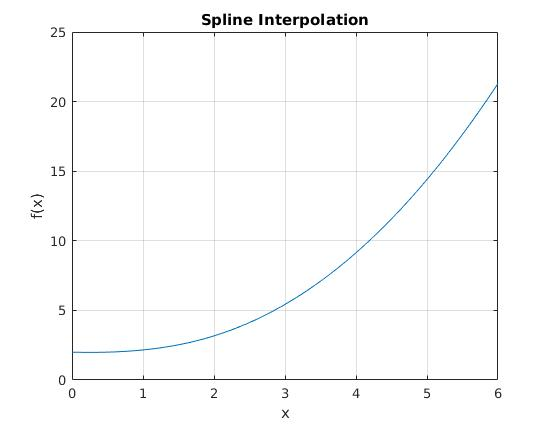
\includegraphics[scale = 0.6]{8_1.jpg}
\caption{Spline Interpolation}
\end{figure}
\newpage

\section{Spline and Quadratic Interpolation}
Carry out a quadratic spline interpolation of the data provided below. Present your result by plotting the spline functions.
\begin{table}[!h]
\begin{tabular}{|c|c|c|c|}\hline
x & -2    & -1    & 0    \\\hline
y & -15 & -8 & -3 \\ \hline
\end{tabular}
\end{table}
\subsection{Plots}
\begin{figure}[!h]
\centering
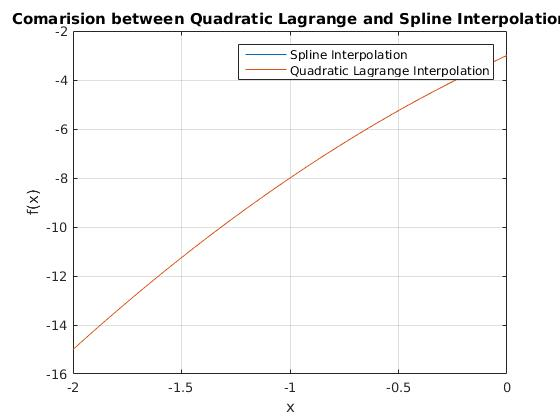
\includegraphics[scale = 0.55]{8_2.jpg}
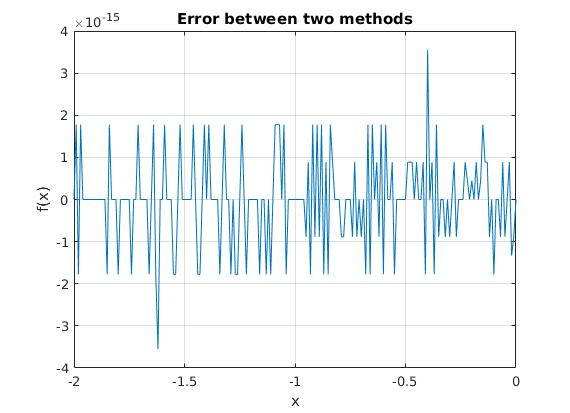
\includegraphics[scale = 0.55]{8_3.jpg}
\caption{Comparison of Linear Piece-wise and Spline}
\end{figure}
\newpage

\section{Numerical Integration}
\subsection{$e^x\cos{4x}$}
Actual Value of the Integral
$$I = \int_{0}^{\pi} e^x\cos{4x} dx = \frac{e^{\pi}-1}{17}$$
\begin{table}[h!]
\centering{\Large
\begin{tabular}{|c|c|c|c|c|}
\hline
$n$   & $T_n$ & $error(T_n)$   & $S_n$  & $error(S_n)$    \\
\hline
2   & 26.516 & 25.214   & 22.715  & 21.413    \\
4   & 3.2491 & 1.9467   & -4.5067 & -5.8091   \\
8   & 1.6245 & 0.32213  & 1.083   & -0.21938  \\
16  & 1.3757 & 0.073329 & 1.2928  & -0.009605 \\
32  & 1.3203 & 0.017918 & 1.3018  & -0.000552 \\
64  & 1.3068 & 0.004454 & 1.3024  & -3.4e-05  \\
128 & 1.3035 & 0.001112 & 1.3024  & -2e-06    \\
256 & 1.3027 & 0.000278 & 1.3024  & 0         \\
512 & 1.3025 & 6.9e-05  & 1.3024  & 0         \\
\hline  
\end{tabular}}
\end{table}
\subsection{$x^{\frac{5}{2}}$}

Actual Value of the Integral
$$I = \int_{0}^{1} x^{\frac{5}{2}} dx = \frac{2}{7}$$
\begin{table}[h!]
\centering{\Large
\begin{tabular}{|c|c|c|c|c|}
\hline
$n$   & $T_n$ & $error(T_n)$   & $S_n$  & $error(S_n)$    \\
\hline
2   & 0.33839 & 0.052674 & 0.28452 & -0.001196 \\
4   & 0.29879 & 0.013077 & 0.28559 & -0.000122 \\
8   & 0.28897 & 0.00326  & 0.2857  & -1.2e-05  \\
16  & 0.28653 & 0.000814 & 0.28571 & -1e-06    \\
32  & 0.28592 & 0.000203 & 0.28571 & 0         \\
64  & 0.28577 & 5.1e-05  & 0.28571 & 0         \\
128 & 0.28573 & 1.3e-05  & 0.28571 & 0         \\
256 & 0.28572 & 3e-06    & 0.28571 & 0         \\
512 & 0.28572 & 1e-06    & 0.28571 & 0 \\
\hline  
\end{tabular}}
\end{table}
\newpage
\subsection{$\frac{1}{1+(x-\pi)^2}$}

Actual Value of the Integral
$$I = \int_{0}^{1} \frac{1}{1+(x-\pi)^2} dx = \arctan{5-\pi} + \arctan{\pi}$$
\begin{table}[h!]
\centering{\Large
\begin{tabular}{|c|c|c|c|c|}
\hline
$n$   & $T_n$ & $error(T_n)$   & $S_n$  & $error(S_n)$    \\
\hline
2   & 2.1667 & -0.17311  & 2.6251 & 0.28533   \\
4   & 2.2687 & -0.071099 & 2.3027 & -0.037094 \\
8   & 2.3323 & -0.007496 & 2.3535 & 0.013705  \\
16  & 2.3378 & -0.001953 & 2.3397 & -0.000106 \\
32  & 2.3393 & -0.000489 & 2.3398 & -1e-06    \\
64  & 2.3396 & -0.000122 & 2.3398 & 0         \\
128 & 2.3397 & -3.1e-05  & 2.3398 & 0         \\
256 & 2.3398 & -8e-06    & 2.3398 & 0         \\
512 & 2.3398 & -2e-06    & 2.3398 & 0      \\
\hline  
\end{tabular}}
\end{table}

\subsection{$e^{-x^2}$}

\begin{table}[h!]
\centering{\Large
\begin{tabular}{|c|c|c|}
\hline
$n$   & $T_n$  & $S_n$     \\
\hline
2   & 2.5     & 1.6667  \\
4   & 1.2548  & 0.83977 \\
8   & 0.88943 & 0.76763 \\
16  & 0.88623 & 0.88516 \\
32  & 0.88623 & 0.88623 \\
64  & 0.88623 & 0.88623 \\
128 & 0.88623 & 0.88623 \\
256 & 0.88623 & 0.88623 \\
512 & 0.88623 & 0.88623 \\
\hline  
\end{tabular}}
\end{table}
\newpage
\subsection{$\arctan{1+x^2}$}

\begin{table}[h!]
\centering{\Large
\begin{tabular}{|c|c|c|}
\hline
$n$   & $T_n$  & $S_n$     \\
\hline
2   & 13.528 & 14.126 \\
4   & 14.231 & 14.466 \\
8   & 14.374 & 14.422 \\
16  & 14.378 & 14.379 \\
32  & 14.378 & 14.378 \\
64  & 14.378 & 14.378 \\
128 & 14.378 & 14.378 \\
256 & 14.378 & 14.378 \\
512 & 14.378 & 14.378 \\
\hline  
\end{tabular}}
\end{table}

\section{Numerical Differentiation}

\subsection{$\arctan{x^2-x+1}$}
$$f'(x) = \frac{2x-1}{1+(x^2-x+1)^2}$$
at $x = 1$, $$f'(1) = \frac{2*1-1}{1+(1^2-1+1)} = \frac{1}{2}$$
\begin{table}[h!]
\centering{\Large
\begin{tabular}{|c|c|c|c|c|}
\hline
$h$   & $D_h$  & $error(D_h)$ & $C_h$ & $error(C_h)$  \\
\hline
0.1     & 0.52086 & 0.020855  & 0.49586 & -0.0041443  \\
0.05    & 0.51146 & 0.01146   & 0.49896 & -0.0010403  \\
0.025   & 0.50599 & 0.0059897 & 0.49974 & -0.00026033 \\
0.0125  & 0.50306 & 0.0030599 & 0.49993 & -6.5099e-05 \\
0.00625 & 0.50155 & 0.0015462 & 0.49998 & -1.6276e-05 \\
\hline  
\end{tabular}}
\end{table}

\newpage
\subsection{$\arctan{100x^2-199x+100}$}
$$f'(x) = \frac{200x-199}{1+(100x^2-199x+100)^2}$$
at $x = 1$, $$f'(1) = \frac{200*1-199}{1+(100*1^2-199+100)} = \frac{1}{2}$$
\begin{table}[h!]
\centering{\Large
\begin{tabular}{|c|c|c|c|c|}
\hline
$h$   & $D_h$  & $error(D_h)$ & $C_h$ & $error(C_h)$  \\
\hline
0.1     & 3.4098  & 2.9098  & 0.20029 & -0.29971   \\
0.05    & 2.5941  & 2.0941  & 0.39043 & -0.10957   \\
0.025   & 1.6757  & 1.1757  & 0.46978 & -0.030224  \\
0.0125  & 1.1093  & 0.60933 & 0.49226 & -0.0077385 \\
0.00625 & 0.80839 & 0.30839 & 0.49805 & -0.0019461\\
\hline  
\end{tabular}}
\end{table}
\subsection{Observation}
\begin{itemize}
    \item We can clearly see that the error of the derivative calculated by the central difference is substantially less than the derivative calculated by the forward difference method on account of the error being proportional to $h^2$ in case of central difference and being proportional to $h$ in case of forward difference.
\end{itemize}

\end{document}